\chapter{Implementation}
\label{implementation}
Machine Learning and especially Deep Learning systems are resource intensive algorithms that need large amounts of both training data and computations. Because the computations needed for ML typically is large matrix operations, it is preferable to run most of the training on GPUs.

\textbf{Edit note: Need more here}

\section{Python}
Python as a programming language choice for Machine Learning is becoming more and more common. It's strength in rapid prototyping and large community that makes troubleshooting easier is heavily outweighed by the slow run time, so while Python out-of-the-box is not suited for these operations, the number of good packages for machine learning and data-processing is quite good and works around Pythons native limitations. 

\subsection{TensorFlow}
TensorFlow\cite{tensorflow} is an open source symbolic math library. It is commonly used for Machine Learning and neural network implementation as it makes it possible to design graph structures in Python. The graphs created operate on n-dimensional matrices called tensors through graphs of mathematical operations and is executed with low-level backend libraries such as \textit{C} or \textit{Fortran}.

TensorFlow also provides the support for different computing devices as needed, meaning the same implementation can be made to run on GPU with excellent benefits to computation time. The implementation used in this thesis runs all model training (weight optimization) on the GPU, but because of the substantial computation performed on the CPU between each model training, the speedup from this is not as substantial as it could be. Future implementations could take advantage of customized graph-nodes to perform tournament searches quicker. 

\subsection{Keras}
Keras\cite{keras} is a high-level Machine Learning API that has a generalized and modular approach to neural network implementation. It depends on a specialized, well-optimized low-level backend library to perform necessary tensor operations and supports the use of TensorFlow, Theano or CNTK backend. Keras provides superior debugging feedback to a stand-alone TensorFlow implementation, while it supports micro-managing of parameters through tensors or matrices.

\begin{figure}[ht]
    \centering
    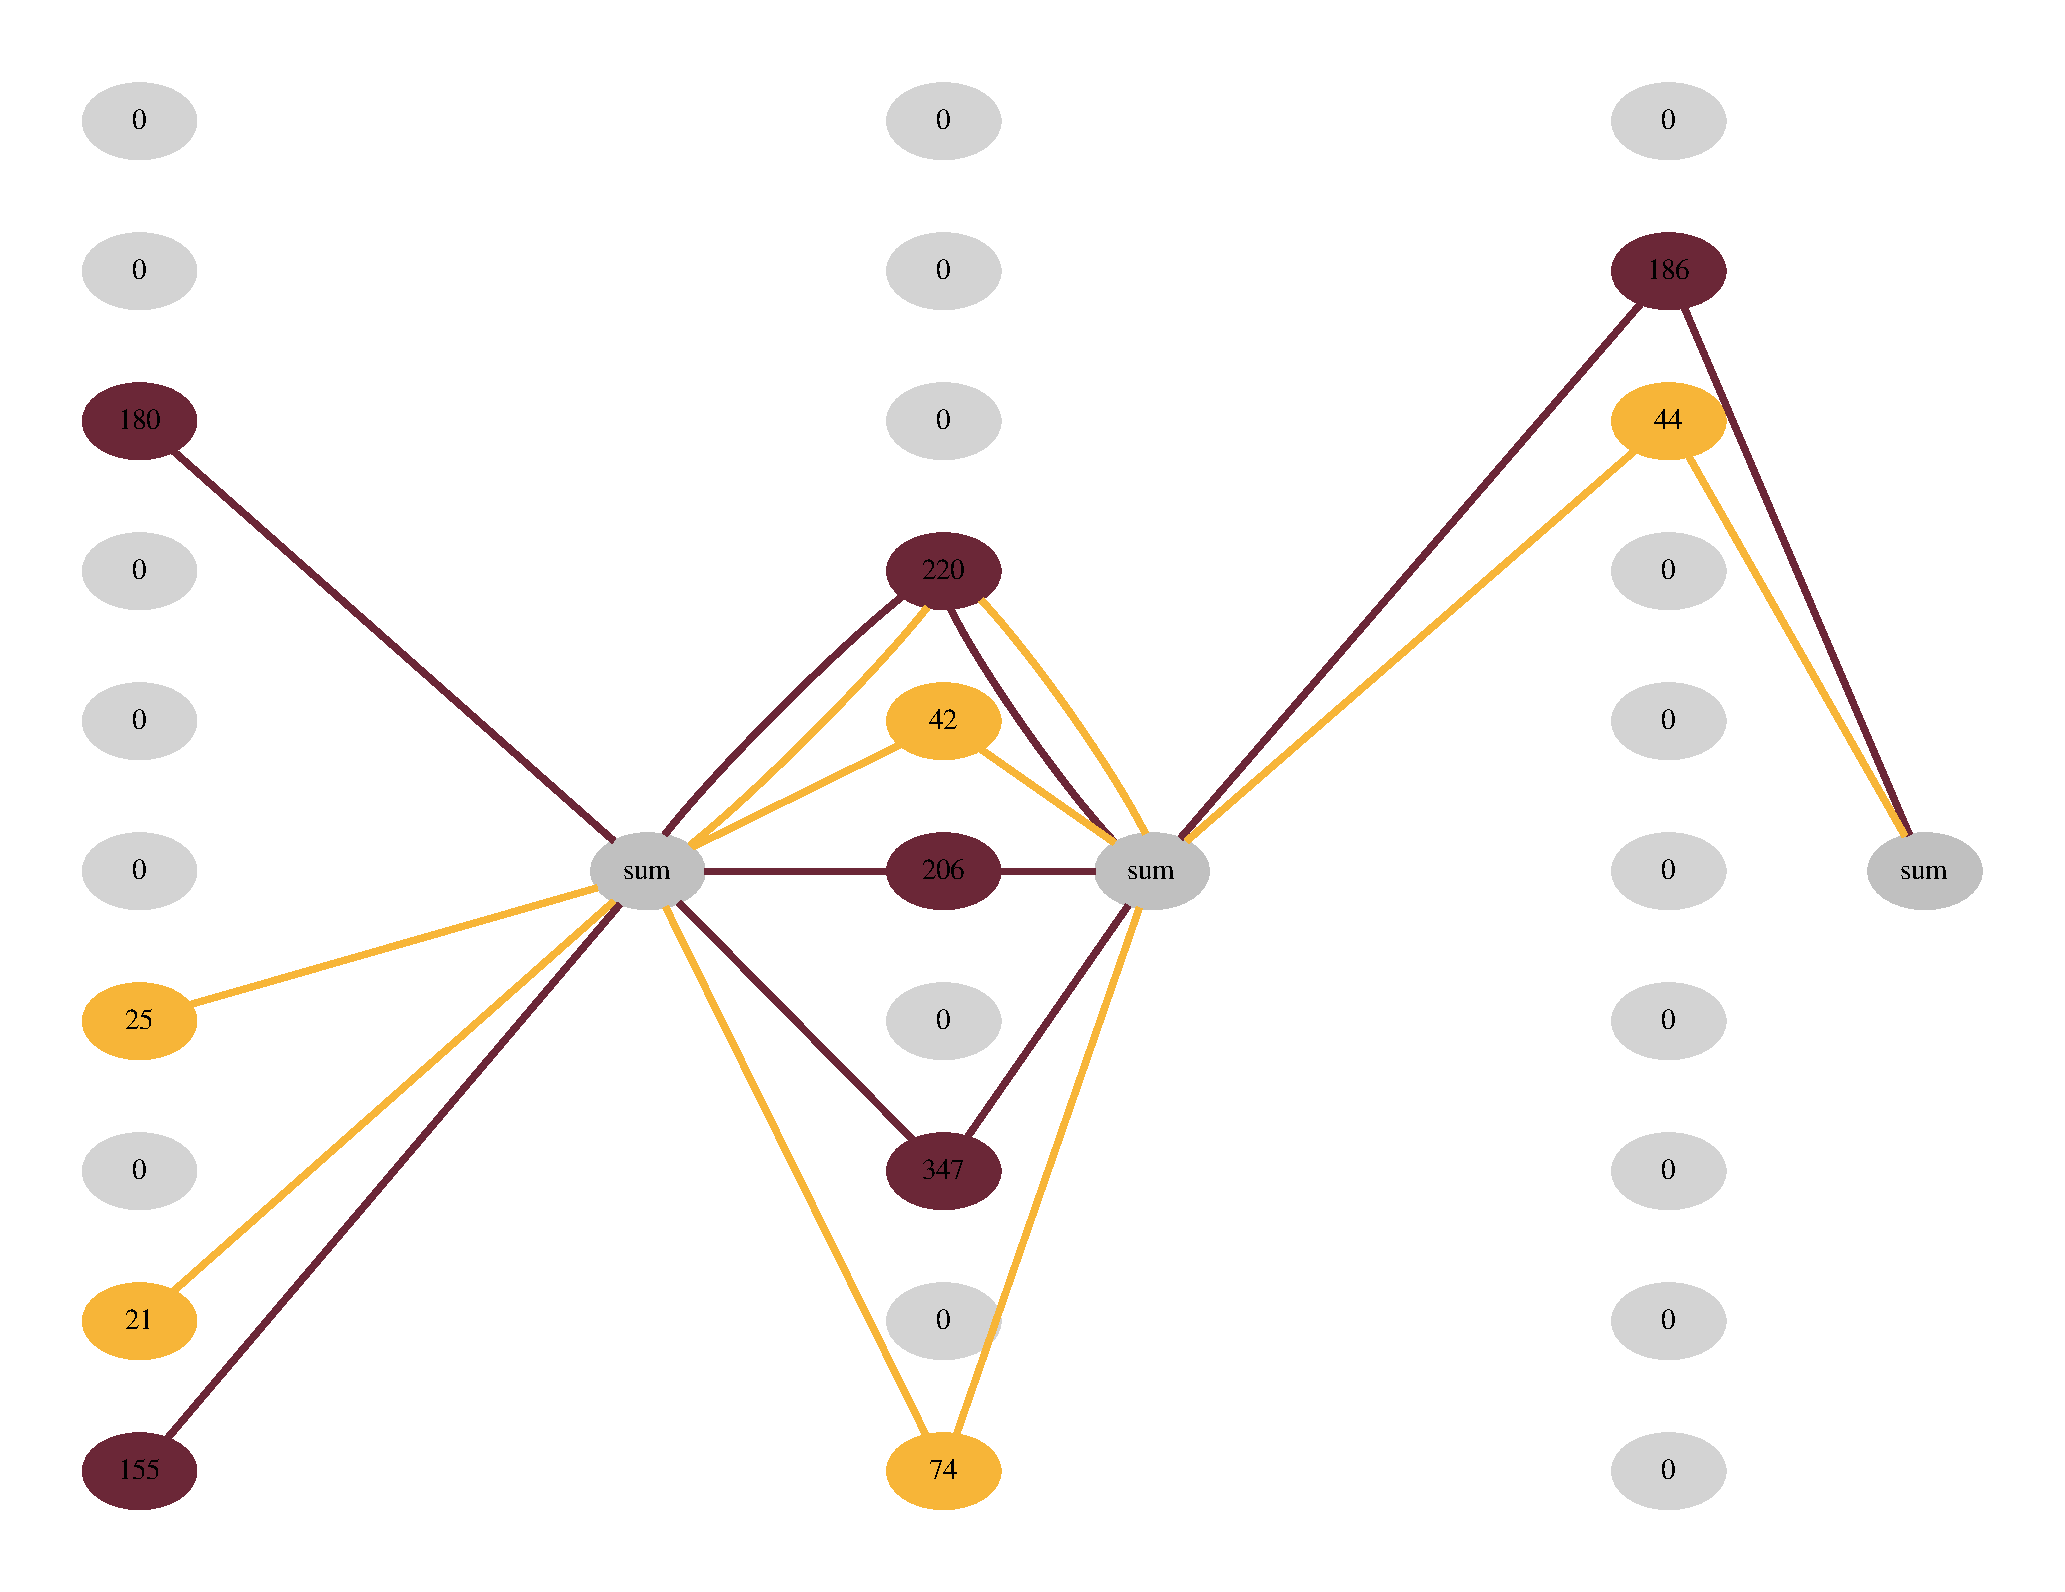
\includegraphics[width=0.8\textwidth]{Chapters/3.Implementation/figures/pathnet_visualization.pdf}
    \caption[GraphViz example]{Graph-visualization of two optimal paths through a PathNet-structure created with GraphViz. This example is of a three-layer PathNet with ten modules in each layer. The first path (red) has a total of 6 modules, and each module contains the number of training units that module have received. The second path (yellow) also use six modules but reuse one module from the first path (second layer, the fourth module from the top). Note that all modules not part of a path (gray) have undergone zero training because the weights have been reinitialized after finding the second path}
    \label{fig:pathnetexample}
\end{figure}

\subsection{Other packages}
Some other mentions to packages used during implementation of this thesis are
\begin{itemize}
    \item SciPy: Providing package containing statistical tests such as the Mann-Whitney-Wilcoxon U-test
    \item Pickle: Used during experimentation to store results and metrics.
    \item Matplotlib: Used for visualization of results.
    \item Numpy: Used for most mathematical operations not available through native Python functions 
    \item GraphViz: Used for generating graphs of PathNet structures for debugging. Multiple paths are drawn in the same graph with training amount in each module as seen in figure \ref{fig:pathnetexample}
    \item Reprint: Used to manage search terminal output by refreshing multi-line output in the terminal.
\end{itemize}

\section{PathNet implementation}
As the same code is used in multiple experiments, it is built to be easily configurable and highly modular. This object-oriented design is based around Keras's already generalized approach to Machine Learning.

\subsection{Code structure}
Modules are implemented through Layer-objects of two types: Dense layers to hold fully-connected modules and Conv layers to hold convolutional modules. Each module type is defined through a configuration-dictionary describing the NN's that constitute a module. 

\begin{lstlisting}[language=Python]
    dense = [{'out': 20, 'activation': 'relu'}, 
             {'out': 5, 'activation': 'softmax'}]
    conv  = [{'channels': 10, 'kernel': (3,3), 
              'stride': (1,1), 'activation':'relu'}]
\end{lstlisting}
In the example above, the two lists yield different module-types. \textit{dense} defines a fully connected NN with two layers, where the first layer have 20 nodes with ReLU activation and the second have a softmax activation. \textit{conv} defines a one layer CNN where the two-dimensional convolution have 10 channels, use a three-by-three kernel with a stride\footnote{As mentioned in section \ref{background:ML}, stride is how far the kernel jumps in each dimension.} of 1 in each dimension and a ReLU activation.

The Layer-objects also define other operations that can be turned on or off on instantiation through parameters. These are:
\begin{itemize}
    \item BatchNormalization\cite{batchnorm} in Conv-modules. This normalizes the output from a layer within each batch. This is to average potential extremes/outliers in input examples to limit radical gradients during training.
    \item MaxPooling used after last Conv-layer. This operation reduces the dimensionality of a layer output by reducing each x-by-y\footnote{Here, only MaxPooling of 2-by-2 windows are performed. This means a 10-by-10 feature map would be reduced to 5-by-5.} window of pixels to the max value within that window.
    \item Flatten before the first Dense-layer. This \textit{"housekeeping"} functionality takes some n-dimensional tensor input and flattens it to a vector to be input into a fully connected NN.  
\end{itemize}

As mentioned in \ref{background:pn}, each task has its unique task-specific final layer that defines the output from PathNet for that task. This concluding layer is defined by task-objects containing one layer of fully connected nodes, an activation function, and output size specific to each task. Only classification is done in this thesis, so all tasks use a softmax activation. These object also contain some meta-info about the model they are a part of, such as input-dimensions, optimizer used for this task, a learning rate, and loss-function. 

The PathNet-object is the only one utilizing the Layer and Task-objects. Through hard-coded static methods, an initialized PathNet structure is created for each experimental run. These methods initialize all layers, modules, and configurations needed to start training. The PathNet-object also contains functionality for generating random paths and Keras-models from a given path-description and task object. It also includes a training counter for each module and an interface for updating this value. There is also some \textit{housekeeping} functionality such as saving and locking modules and a TensorFlow-session backend reset (see section \ref{implementation:problems}).

\section{Search implementation}
\label{implementation.search}
As with PathNet, the search has a modular implementation for easy adaptability and reuse in all experiments. Based on a hyper-parameter dictionary, the search method uses predetermined functions for different GA operations, such as selection-schemes for winner selection or path mutation. The selection-schemes used is winner-replace-all, where a mutation of the winner replace all other genomes in the tournament, and a 3-to-2 scheme where the two winners of a tournament size of 3 are recombined and the offspring replace the tournament looser.

Every generation updates a Reprint-structure that gives terminal output of the search progress (see figure \ref{fig:searchoutput} for screen capture of a experimental run).
\begin{figure}[ht]
    \centering
    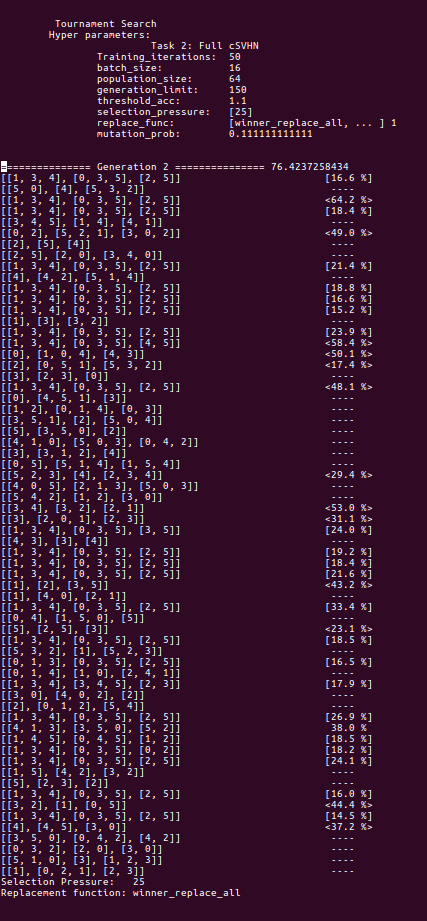
\includegraphics[width=0.6\textwidth]{Chapters/3.Implementation/figures/search_output.png}
    \caption[Terminal search output]{Screen shot of terminal output during a search. The top section contains hyper-parameters for this search as well as current generation number. Underneath the current population-state can be seen as well as some accuracies in the right margin. For these, \big[ \big] means the accuracy is outdated by training, \big< \big> means the value within is a training accuracy, .... means the path is not evaluated yet, and a plain percentage is the actual fitness of that path. At the bottom, the current generations selection pressure is printed, as well as the selection scheme.}
    \label{fig:searchoutput}
\end{figure}
\textbf{Edit note: Need more?}

\section{Notable implementation differences}
\begin{itemize}
    \item Implementation is built upon the Keras API and is more modular in its object-oriented structure
    \item Path fitness is not the negative error, but classification accuracy. 
    \item For the variable selection pressure experiment, the fitness calculation is performed after a separate training step. See \ref{exp2:implementation} for details and reasoning.
\end{itemize}

\section{Implementation difficulties} 
\label{implementation:problems}
Some implementation difficulties occurred during implementation. Most of these were due to TensorFlow effect I was unaware of. Some of the most noteworthy are listed here to help with future implementation.
\begin{itemize}
    \item The TensorFlow backend session is not made for creating multiple graphs, and memory leaks can happen when memory used for graphs is not freed properly. Functionality in TensorFlow makes it possible to reset a TensorFlow session, but all graph-variables has to be reinitialized afterward. 
    \item TensorFlow's default is to use all available GPU-memory. Setting the TensorFlow-sessions GPU-options "allow-growth" parameter to 4 sets memory allocation to be done as needed.
    \item Allocated memory is not freed by TensorFlow until the Python process that initialized it is ended.
\end{itemize}

\section{Data sets}
\subsection{MNIST}\label{Implementation:MNIST}
One of the most commonly used data sets for image classification is the MNIST\cite{MNIST} set of hand-drawn digits. These 28 by 28 grayscale images contain one digit from 0 through 9 each. The 60 000  labeled images are distributed about evenly across all ten classes. 

\begin{figure}[p!]
    \centering
    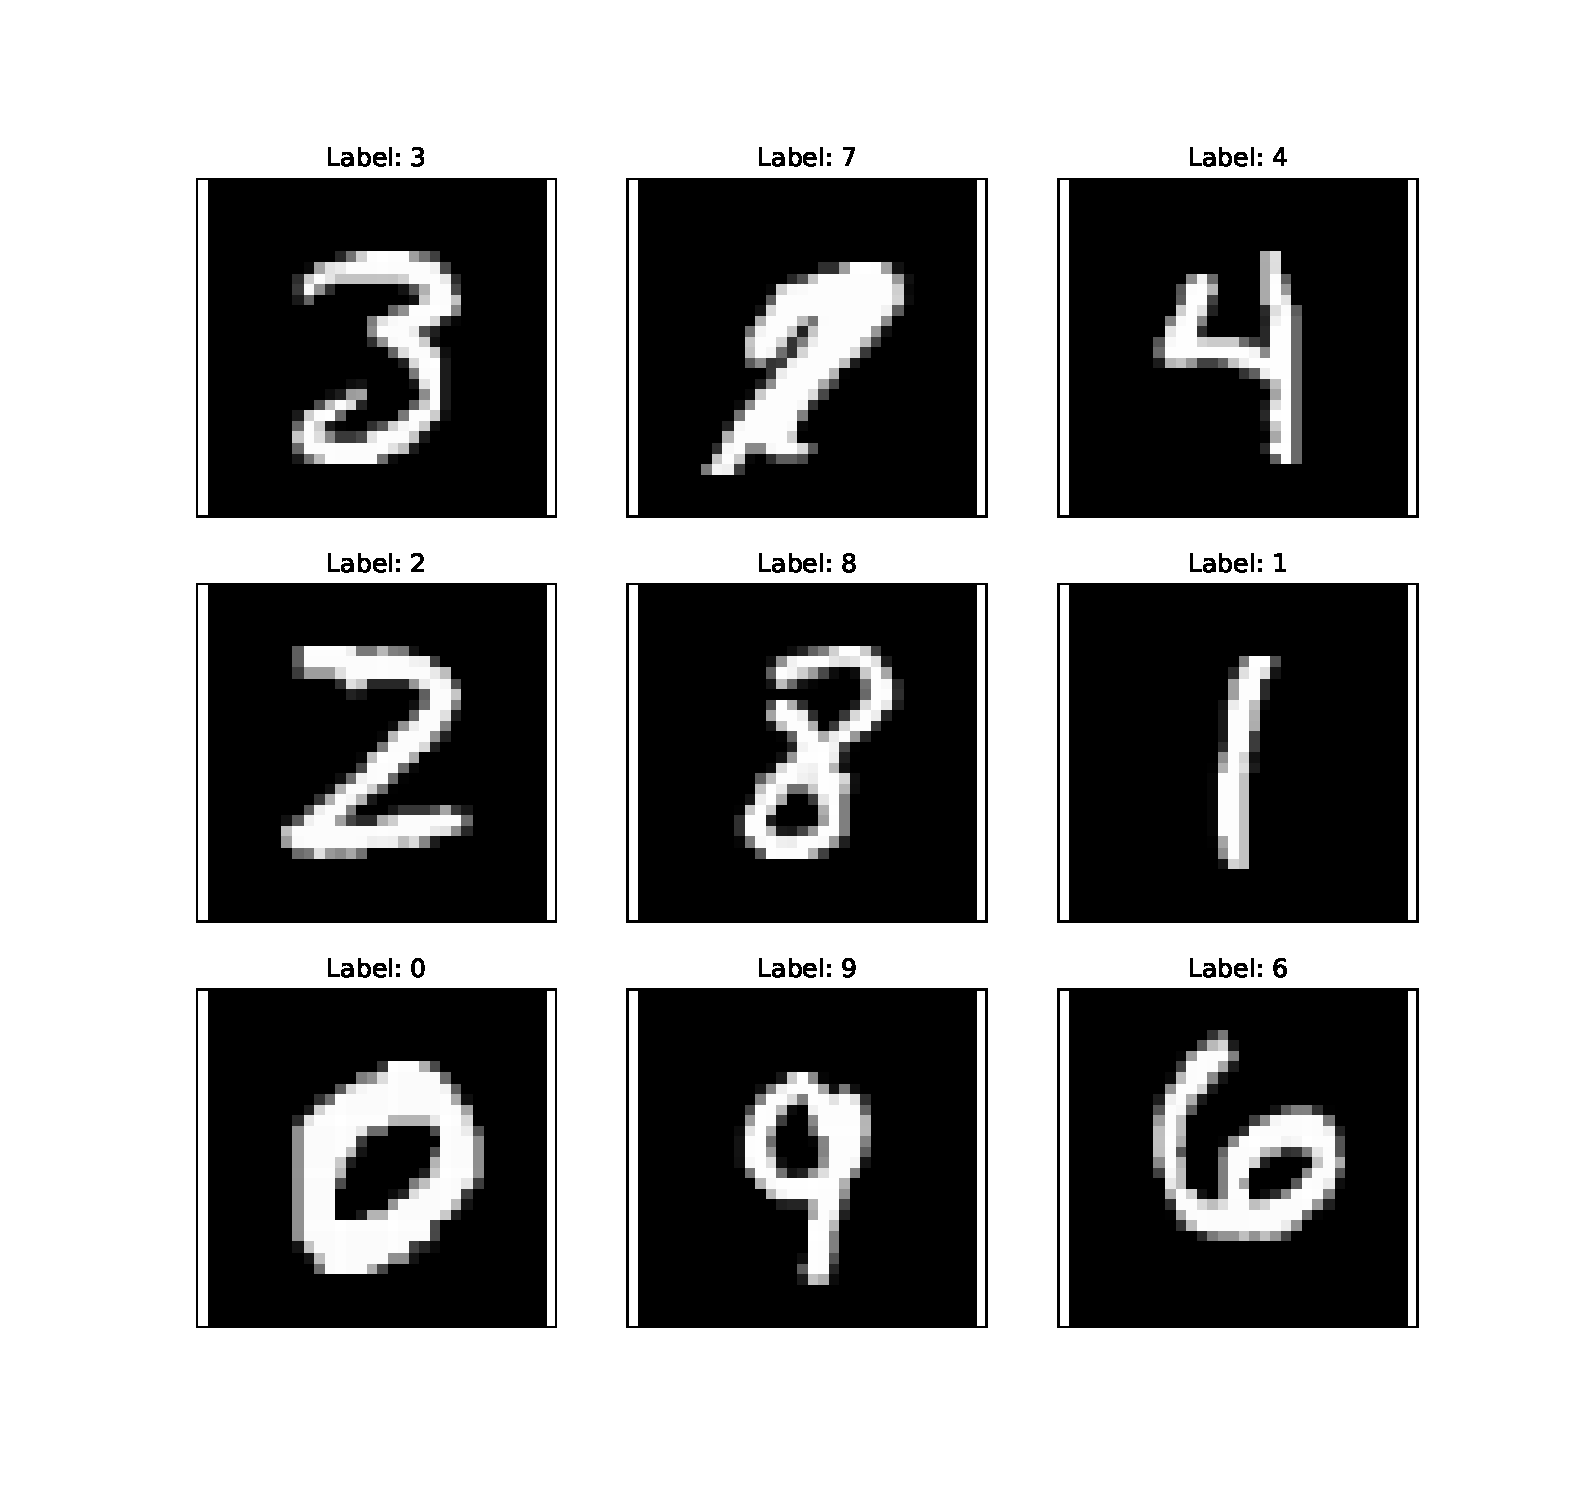
\includegraphics[width=0.8\textwidth]{Chapters/3.Implementation/figures/MNIST.pdf}
    \caption[MNIST example]{Nine images from the MNIST data set.}
    \label{fig:mnist}
\end{figure}

MNIST is a simple data set as far as image classification goes (see section \ref{exp1:BIN.results}). The small grayscale images contain only one small object in the middle of the image, and almost all pixels is either 0 (background) or 1 as seen in figure \ref{fig:mnist}. This makes the classification task rather easy. A list of reached accuracies\footnote{As of March 2018} can be found on the dataset's web page where it is claimed that the lowest error rate is 0.23\cite{goodmnist}, and even a KNN-classifier without preprocessing can achieve an accuracy of 97.17. 


\subsection{SVHN}\label{Implementation:SVHN}
The Street View House Number\cite{SVHN} data set is real-world images from Google Street View made for machine learning development. The original dataset contains over 600 000 variable resolution images of house numbers and bounding boxes around each digit with a label for each box. In this thesis, the version of SVHN used is made of cropped images (cSVHN) as seen in figure \ref{fig:csvhn}. These images are 32-by-32 colored images that are made to function in somewhat the same way MNIST does, with a simple object and static size. Note, however, that where MNIST images contain only the object that is the basis for classification, cSVHN contain distractions (noise) in the image such as half-cropped neighbouring digits. 

\begin{figure}[p!]
    \centering
    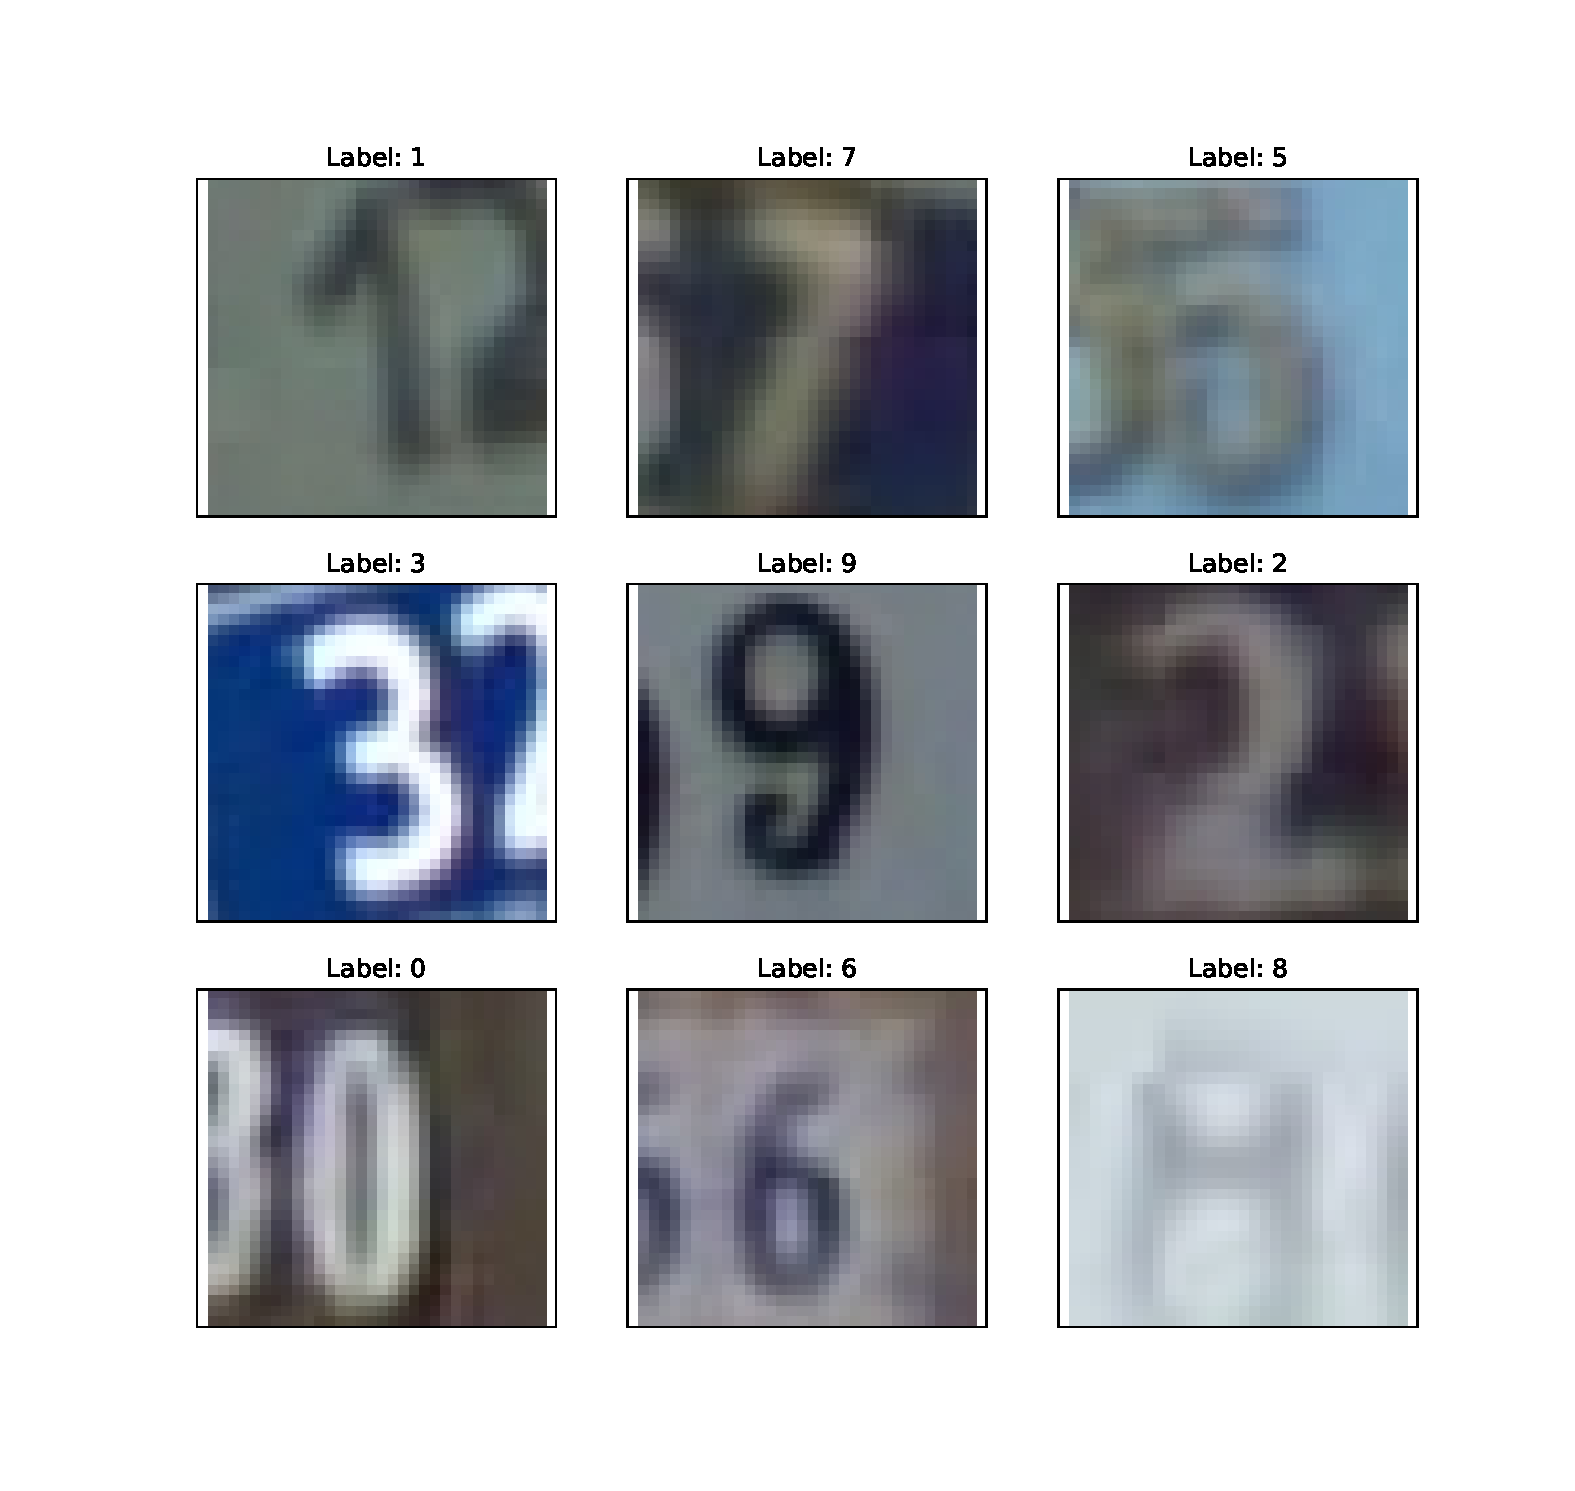
\includegraphics[width=0.8\textwidth]{Chapters/3.Implementation/figures/cSVHN.pdf}
    \caption[cSVHN example]{Nine images from the cSVHN data set.}
    \label{fig:csvhn}
\end{figure}

The whole image set is split into three sets, a training set containing 73257 digits, a test set of 26032 digits, and a simplified \textit{"extra"} image set of 531131 images, claimed by the creator to be "less difficult." This extra, simplified image set is the one used in the experiments in chapter \ref{exp2} for task 3a, 3b, and 4 and both tasks in chapter \ref{exp3}.

\begin{table}[h]
    \centering
    \begin{tabular}{ccc}
    Class number (Digit) & Number of samples & \% of whole data set\\
    0                    & 45550             & 8.6\%               \\
    1                    & 90560             & 17.0\%              \\
    2                    & 74740             & 14.1\%              \\
    3                    & 60765             & 11.5\%              \\
    4                    & 50633             & 9.5\%               \\
    5                    & 53490             & 10.1\%              \\
    6                    & 41582             & 7.8\%               \\
    7                    & 43997             & 8.3\%               \\
    8                    & 35358             & 6.7\%               \\
    9                    & 34456             & 6.5\%              
    \end{tabular}
    \caption{Distribution of samples on each class in the cropped SVHN set used in this thesis, along with the portion of the whole set each class constitute. Given a random selection of samples from this set, this percentage should approximately be the probability of selection each class}
    \label{tab:SVHN}
\end{table} 

Because these images are from the real world, and because of the nature of house numbers, the class distribution is not even. In table \ref{tab:SVHN} the number of digits in each class in the extra set is listed along with the portion of the whole set this constitutes.  

\iffalse
    X   Can you describe your implementation in detail? 
    X   Why did you use this technology? 
    X   How does the theory relate to your implementation? 
    X   What are your underlying assumptions? 
    X   What did you neglect and what simplifications have you made? 
    X   What tools and methods did you use? 
    X   Why use these tools and methods? 
\fi